%===============================================================
%Template for UPC-TALP based on CTU and modified to match UPC-TALP colors and style  
%The original template from Czech Technical University  % Author: Martin Malý.
% They are defined by new graphical manual - 2017.
% Share and modify as you like. Keep the name of the authors.
% It is forbidden to use the template commercially.
%===============================================================

\documentclass{beamer}
\usepackage[utf8]{inputenc}
%\usepackage{lmodern}

\usepackage{comment}
\usetheme{Madrid}
  \usepackage[maxbibnames=99]{biblatex}
\definecolor{cvut_navy}{HTML}{0065BD}
\definecolor{cvut_blue}{HTML}{6AADE4}
\definecolor{cvut_gray}{HTML}{156570}
\usepackage{biblatex}
%\usepackage{tikz}
%\usepackage{pgfplots}
\usepackage[makeroom]{cancel}
\usepackage{threeparttable}
\usepackage[utf8]{inputenc}
%\usepackage[usenames,dvipsnames]{xcolor}
%\addbibresource{biblatex-examples.bib}
%\setbeamercolor{section in toc}{}
\setbeamercolor{section in toc}{fg=black,bg=yellow} 
\setbeamercolor{alerted text}{fg=cvut_blue}
\usepackage{tikzsymbols}
\usepackage{textcomp}
\usepackage{parskip}
\definecolor{darkblue}{rgb}{0, 0, 0.5} 
\definecolor{babyblue}{rgb}{0.54, 0.81, 0.94}
\usepackage{pgf}
\usepackage{color,soul}
%\usepackage{pythontex} 
\usepackage{tcolorbox}
\tcbuselibrary{skins}
\usepackage{minted}
\usepackage{hyperref}
\usepackage{xcolor,soul}
\definecolor{lightblue}{rgb}{.90,.95,1}
\sethlcolor{lightblue}
\renewcommand<>{\hl}[1]{\only#2{\beameroriginal{\hl}}{#1}}
\setbeamertemplate{page number in head/foot}[framenumber]
%%% attravive box over equestion
\usepackage{empheq}
\usepackage{xcolor}
\definecolor{lightgreen}{HTML}{90EE90}
\newcommand{\boxedeq}[2]{\begin{empheq}[box={\fboxsep=6pt\fbox}]{align}\label{#1}#2\end{empheq}}
\newcommand{\coloredeq}[2]{\begin{empheq}[box=\colorbox{lightgreen}]{align}\label{#1}#2\end{empheq}}
\newcommand{\highlight}[1]{%
  \colorbox{red!40}{$\displaystyle#1$}}
  
  
  \definecolor{babyblue}{rgb}{0.54, 0.81, 0.94}
\definecolor{babypink}{rgb}{0.96, 0.76, 0.76}
\definecolor{blue(ncs)}{rgb}{0.0, 0.53, 0.74}
\definecolor{pistachio}{rgb}{0.58, 0.77, 0.45}
\definecolor{darksalmon}{rgb}{0.91, 0.59, 0.48}
\definecolor{lightsalmonpink}{rgb}{1.0, 0.6, 0.6}
\definecolor{columbiablue}{rgb}{0.61, 0.87, 1.0}
\definecolor{corn}{rgb}{0.98, 0.93, 0.36}
\definecolor{jonquil}{rgb}{0.98, 0.85, 0.37}
\definecolor{bananayellow}{rgb}{1.0, 0.88, 0.21}
\newcommand{\bert}{\ensuremath{%
  \mathchoice{\includegraphics[height=2ex]{Bert-pic-removebg-preview.png}} 
    {\includegraphics[height=2ex]{Bert-pic-removebg-preview.png}}
    {\includegraphics[height=1.5ex]{Bert-pic-removebg-preview.png}}
    {\includegraphics[height=1ex]{Bert-pic-removebg-preview.png}}
}}
  
  
\useoutertheme{infolines}



\usepackage{courier}
%\usepackage{animate}  
\usepackage{expl3}
%\usepackage[listings,theorems]{tcolorbox}



%%%%%%%%%%%%%%%%%%%%%%%%%%%%%%%%%%%%%%%%%%%%%%%%%%%%%%%%%%%%%%%%%%%%%  
%commands for simulating terminal in/output  
%\scroll[<line separator string>]{<width as TeX dim>} 
%                             {<number of lines>}{terminal text line}  
%\clearbuf  %clears line buffer  
%%%%%%%%%%%%%%%%%%%%%%%%%%%%%%%%%%%%%%%%%%%%%%%%%%%%%%%%%%%%%%%%%%%%%  



\newcommand\scroll[4][§§]{
  \seq_set_split:Nnn\g_inputline_seq{#1}{#4}
  \seq_map_inline:Nn\g_inputline_seq{
    \seq_gput_right:Nx\g_linebuffer_seq{##1}
    \int_compare:nT{\seq_count:N\g_linebuffer_seq>#3}{
      \seq_gpop_left:NN\g_linebuffer_seq\dummy
    }
  }
  \fbox{\begin{minipage}[t][#3\baselineskip]{#2}
    \ttfamily
    \seq_map_inline:Nn\g_linebuffer_seq{\mbox{##1}\\}
  \end{minipage}}
}
\newcommand\clearbuf{\seq_gclear:N\g_linebuffer_seq}
\ExplSyntaxOff

\setbeamertemplate{headline}{%
\begin{beamercolorbox}[colsep=1.5pt]{upper separation line head}
\end{beamercolorbox}
\begin{beamercolorbox}{section in head/foot}
    \vskip2pt\insertsectionnavigationhorizontal{\paperwidth}{}{\hskip0pt plus1filll}\vskip2pt
\end{beamercolorbox}%

\begin{beamercolorbox}[colsep=1.5pt]{lower separation line head}
\end{beamercolorbox}
}
\makeatletter
\newcommand\SoulColor{%
  \let\set@color\beamerorig@set@color
  \let\reset@color\beamerorig@reset@color}
\makeatother
\SoulColor
\usepackage{amsmath, bm}
\usepackage{tikz}
\setbeamercovered{dynamic}

\newcommand{\highlightt}[1]{%
  \colorbox{blue!40}{$\displaystyle#1$}}


\newenvironment<>{problock}[1]{%
  \begin{actionenv}#2%
      \def\insertblocktitle{#1}%
      \par%
      \mode<presentation>{%
       % \setbeamercolor{block title}{fg=white,bg=orange!20!black}
        %\setbeamercolor{block title}{fg=white,bg=red!10!black}
        \setbeamercolor{block title}{fg=white,bg=cvut_blue}
       \setbeamercolor{block body}{fg=black,bg=white!50}
       \setbeamercolor{itemize item}{fg=orange!20!black}
       \setbeamertemplate{itemize item}[triangle]
     }%
      \usebeamertemplate{block begin}
    \par\usebeamertemplate{block end}
    \end{actionenv}
    }
    
    \newcommand<>{\uncovergraphics}[2][{}]{
    % Taken from: <https://tex.stackexchange.com/a/354033/95423>
    \begin{tikzpicture}
    \node[anchor=south west,inner sep=0] (B) at (4,0)
        {\includegraphics[#1]{#2}};
    \alt#3{}{%
        \fill [draw=none, fill=background, fill opacity=0.9] (B.north west) -- (B.north east) -- (B.south east) -- (B.south west) -- (B.north west) -- cycle;
    }
    \end{tikzpicture}
}




\newlength\dlf
\newcommand\alignedbox[3][yellow]{
  % #1 = color (optional, defaults to yellow)
  % #2 = before alignment
  % #3 = after alignment
  &
  \begingroup
  \settowidth\dlf{$\displaystyle #2$}
  \addtolength\dlf{\fboxsep+\fboxrule}
  \hspace{-\dlf}
  \fcolorbox{red}{#1}{$\displaystyle #2 #3$}
  \endgroup
}

\usepackage{collcell}
\usepackage{booktabs}
\usepackage{etoolbox}
%\usepackage{remreset}% tiny package containing just the \@removefromreset command
\makeatletter

\usepackage{xcoffins}
\NewCoffin\tablecoffin
\NewDocumentCommand\Vcentre{m}
  {%
    \SetHorizontalCoffin\tablecoffin{#1}%
    \TypesetCoffin\tablecoffin[l,vc]%
  }



\usepackage{pgfpages}

%% Important 
%%% show note or disable note. 
%\setbeameroption{show notes on second screen=right} % Both

\setbeamertemplate{note page}{\pagecolor{gray!5}\insertnote}\usepackage{palatino}



%\setbeamertemplate{footline}{}
%\setbeamertemplate{footline}{}
\usepackage{xcolor}
\usepackage{soul}

\usepackage{etoolbox}
\makeatletter
%\patchcmd{\slideentry}{\ifnum#2>0}{\ifnum2>0}{}{\@error{unable to patch}}% replace the subsection number test with a test that always returns true
\makeatother

\setbeamercolor*{palette primary}{bg=cvut_navy,fg=gray!20!white}
\setbeamercolor*{palette secondary}{bg=cvut_navy,fg=gray!20!white} % no color
%\setbeamercolor*{palette secondary}{bg=cvut_navy,fg=cvut_navy}
%\setbeamercolor*{palette secondary}{bg=cvut_blue,fg=white}
\setbeamercolor*{palette tertiary}{parent=palette primary} % color of the top and date
\setbeamercolor*{palette quaternary}{fg=cvut_navy,bg=gray!5!white}
\setbeamercolor*{sidebar}{fg=cvut_navy,bg=gray!15!white}
\usepackage[first=0,last=9]{lcg}
\newcommand{\ra}{\rand0.\arabic{rand}}
\usepackage{color, colortbl}
\usepackage{stackengine,tikz}
\usepackage{transparent}
\usepackage{pgfpages}
%\usepackage{graphicx}% http://ctan.org/pkg/graphicx
\usepackage{booktabs}% http://ctan.org/pkg/booktabs
%\setbeameroption{show notes}
\colorlet{Gray}{gray!30}




    
\newcommand*{\MinNumber}{0}%
%\newcommand*{\MaxNumber}{100}%
\newcommand*{\MaxNumber}{0.4}%
\definecolor{bubblegum}{rgb}{0.99, 0.76, 0.8}
\newcommand{\ApplyGradient}[1]{%
  \pgfmathsetmacro{\PercentColor}{100.0*(#1-\MinNumber)/(\MaxNumber-\MinNumber)}%
  %\textcolor{black!\PercentColor}{#1}
  \edef\x{\noexpand\cellcolor{babyblue!\PercentColor}}\x\textcolor{black}{#1}%
}
\newcolumntype{R}{>{\collectcell\ApplyGradient}{c}<{\endcollectcell}}

%\setbeameroption{show notes on second screen=right}
\setbeamercolor{titlelike}{parent=palette primary}
\setbeamercolor{frametitle}{parent=palette primary}

\setbeamercolor{B}{bg=red!30,fg=black}


\setbeamertemplate{section in toc}[default]
\setbeamercolor{itemize item }{fg=blue}
\setbeamertemplate{itemize item}[circle]

\setbeamercolor*{separation line}{}
\setbeamercolor*{fine separation line}{}

\setbeamertemplate{navigation symbols}{} 
\setbeamertemplate{caption}{\raggedright\insertcaption\par}

%\setbeamercolor*{block title example}{fg=blue!50,bg= blue!10}

%\setbeamercolor*{block title example}{fg=white,bg= cvut_navy}
\setbeamercolor*{block title example}{fg=white,bg=purple!75!black}
\setbeamercolor*{block body example}{fg= black, bg= white}


\setbeamercolor{itemize item}{fg=cvut_navy} % all frames will have red bullets
\setbeamercolor{block title}{bg=red!30,fg=black}
\setbeamertemplate{subsection in toc}[subsections numbered]


\usepackage{eqnarray,amsmath}
\usepackage{amsfonts}
\usepackage{amssymb}
\usefonttheme{professionalfonts}
\usepackage{graphicx}
\usepackage{booktabs} 
\usepackage{bm}
\usepackage{mathtools}
\usepackage[utf8]{inputenc}
\usepackage[T1]{fontenc}
\usepackage{lmodern} 
\usepackage{booktabs}


%\setbeamercolor{block title}{fg=darkred,bg=structure.fg!10!bg!10!bg}
%\setbeamercolor{block body}{use=block title,bg=block title.bg}
\definecolor{NormalBlue}{RGB}{200,200,255}
%\setbeamercolor{block title}{bg=NormalBlue}yellow
\setbeamercolor{block title}{fg=black, bg=yellow}
\setbeamercolor{block2}{use=structure,fg=white,bg=purple!75!black}
% definice makra
\def\bq{\mbox{\kern.1ex\protect\raisebox{-1.3ex}[0pt][0pt]{''}\kern-.1ex}}
\def\eq{\mbox{\kern-.1ex``\kern.1ex}}
\def\ifundefined#1{\expandafter\ifx\csname#1\endcsname\relax }%
\ifundefined{uv}%
        \gdef\uv#1{\bq #1\eq}
\fi


%====================================================
%========== DEFINITION OF AUTHORS ETC...=============
%====================================================
\author[Thesis Defense]{Author}
\institute[]{Universitat Politècnica de Catalunya \\  Department of Computer Science
\vspace{2mm} \\ 
Advisors:  \\ Prof. John 
%Dr. Marina \\ 
\vspace{2mm}}
\title[]{Presentation Title}


  \date[March 31, 2023]{\small{Thesis Defense} \\ \small{March 31, 2023}}
%====================================================
%========== BEGINNING OF DOCUMENT ===================
%====================================================


\begin{document}
%\begin{frame}[plain]
%%\transboxin
%
%	\titlepage
%	\begin{center}%
%	%\vspace{-2mm}
%	%\tableofcontents{current}
%  		
\includegraphics[height=1cm]{darkblue-logo.pdf}
%  		%\includegraphics[height=1cm]{darkblue-talp-logo.pdf}
%  		%\includegraphics[height=1.5cm]{upclogo.pdf}
%		%\includegraphics[height=1.1cm]{files/IRIS.png}
%		%\includegraphics[height=1.3cm]{files/logo_iri2.png}https://www.overleaf.com/project/5bed4779c7eea31291e7e8b2#Navigation27
%	%\includegraphics[height=1.3cm]{files/IBT.png}
%		%\includegraphics[height=1.3cm]{files/biocev-logo-CMYK-horizontal.pdf}
%	\end{center}
%%\note[item]{you  note here}
%\end{frame}


%\logo{\includegraphics[height=1cm]{files/TALP.png}}
%\logo{
\includegraphics[height=0.6cm]{darkblue-logo.pdf}}
%\logo{
\includegraphics[height=0.5cm]{darkblue-logo.pdf}}




%\begin{frame}[plain]{Table of Contents}
%     \tableofcontents[currentsection]
%\end{frame}


%\begin{frame}[plain]{Table of Contents}
%\tableofcontents[]
%\note[item]{note here }
%\end{frame}



%\section{Introduction}



%\section{Problem Identification}

%\begin{frame}
%
%	\frametitle{Some Features}
%
%
%\begin{block}<0>
%
%\begin{itemize}
%\item [A] This is the first important point.
%\end{itemize}
%
%\end{block}
%
%\begin{block}<0>
%
%\begin{itemize}
%
%\item [B]  This is the first important point.
%\end{itemize}
%
%\end{block}
%
%\uncover<1>{
%}
%\vspace{-0.1cm}
%
%\end{frame}
%
%
%\begin{frame}
%
%	\frametitle{Highlight with a block}
%
%
%\begin{block}{}
%
%\begin{itemize}
%\item [A] This is the first important point.
%
%\end{itemize}
%
%\end{block}
%
%\begin{block}<0>
%
%\begin{itemize}
%
%\item [B] This is the first important point.
%
%\end{itemize}
%
%\end{block}
%
%
%
%\vspace{0.1cm}
%
%
%\end{frame}
%
%
% \begin{frame}[noframenumbering]{Some Features}
%  \begin{alertblock}
%
%\begin{itemize}
%    \item [A] This is the first important point.
%
%\end{itemize}
%\end{alertblock}
%\visible<2->{
%\begin{alertblock}{\small}
%\begin{itemize}
%
%\item [B] This is the first important point.
%
%\end{itemize}
%\end{alertblock}
%}
%\visible<3->{
%\begin{alertblock}{\small}
%\begin{itemize}
%
%\item [C] This is the first important point.
%
%\end{itemize}
%\end{alertblock}
%}
%
%\visible<4->{
%\begin{alertblock}{\small}
%\begin{itemize}
%
%\item [D] This is the first important point.
%\end{itemize}
%\end{alertblock}
%}
%
%
%
%\end{frame}

\BLOCK{for index, row in data_answers.iterrows()}
\begin{frame}%[noframenumbering]
\frametitle{Unrelated Title}
\begin{itemize}

\BLOCK{for bullet_point in row['answer']}
\item \VAR{bullet_point}
\BLOCK{endfor}

\end{itemize}

%\begin{figure}
%\begin{center}
%
%%%%\vspace{10pt}
%%\vspace{-0.3cm}
%\vspace{0.2cm}
%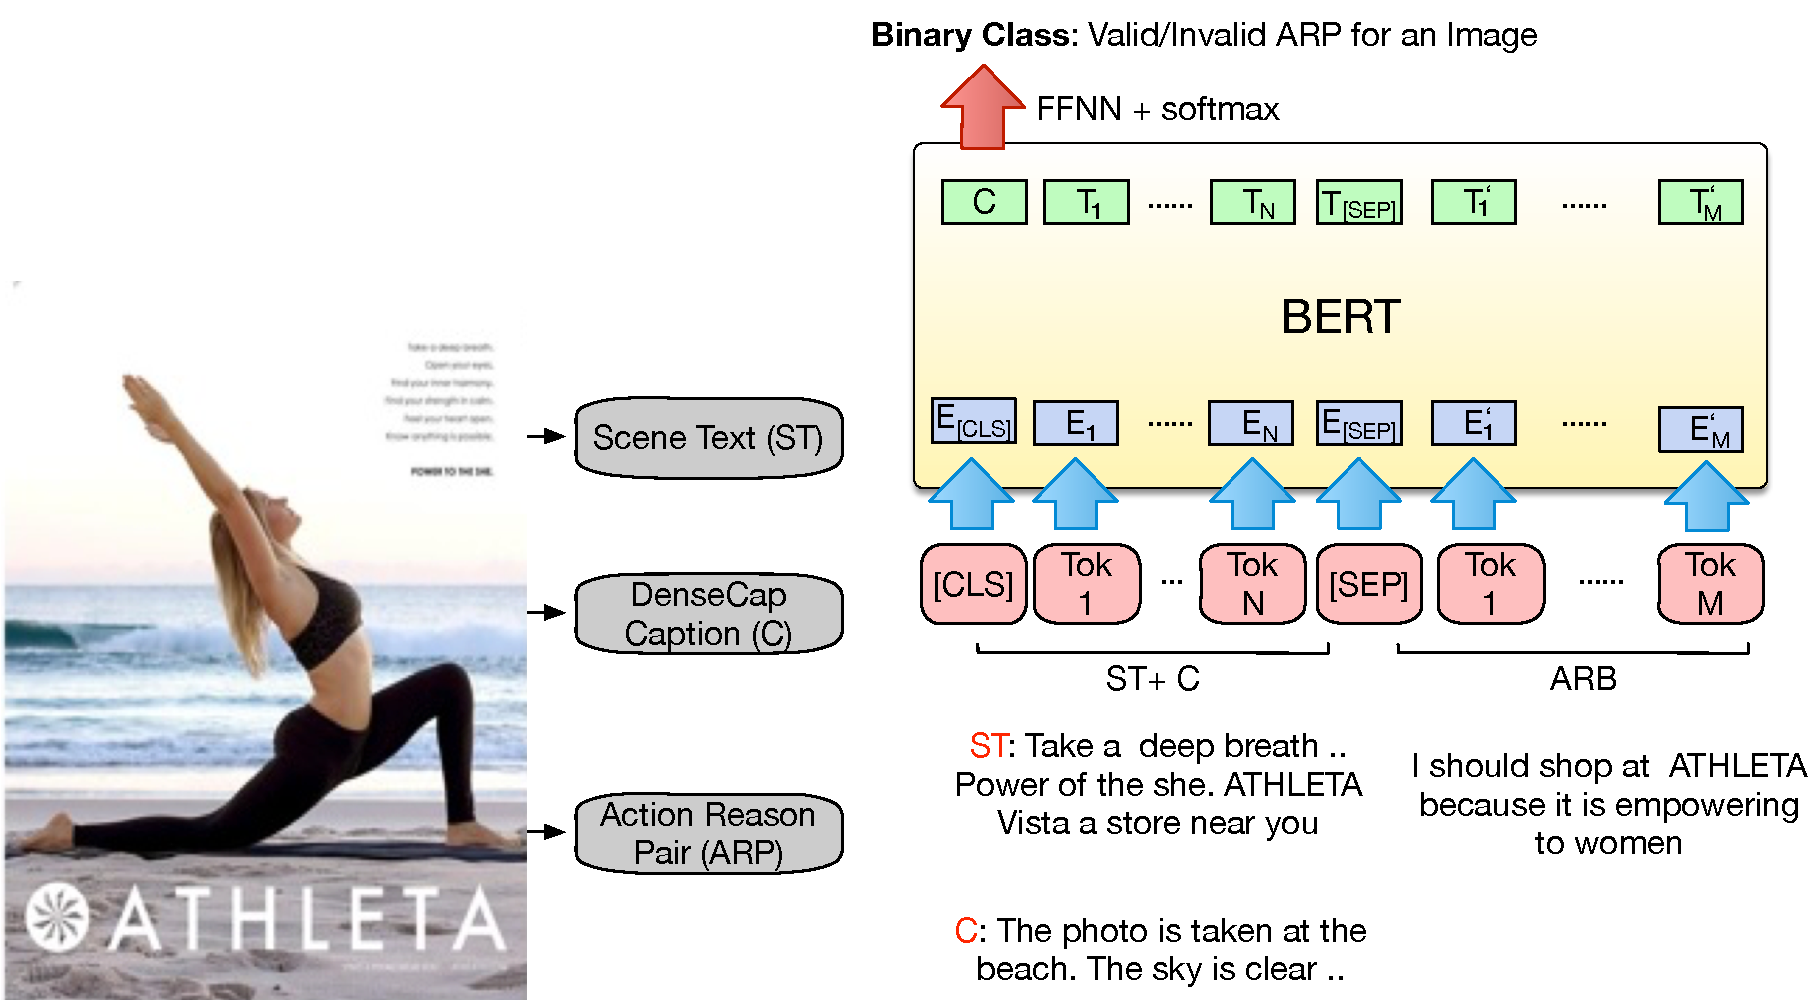
\includegraphics[width=0.6\textwidth]{BERT-2020.pdf}
%
%
%    \label{ActionButton}
%  \end{center}
%\end{figure}
\note[item]{}
\end{frame}
\BLOCK{endfor}

% Images
\BLOCK{for index, row in data_images.iterrows()}
\begin{frame}%[noframenumbering]
\frametitle{Unrelated Title}

\begin{center}
\VAR{row["images"]}
\end{center}
%\begin{figure}
%\begin{center}
%
%%%%\vspace{10pt}
%%\vspace{-0.3cm}
%\vspace{0.2cm}
%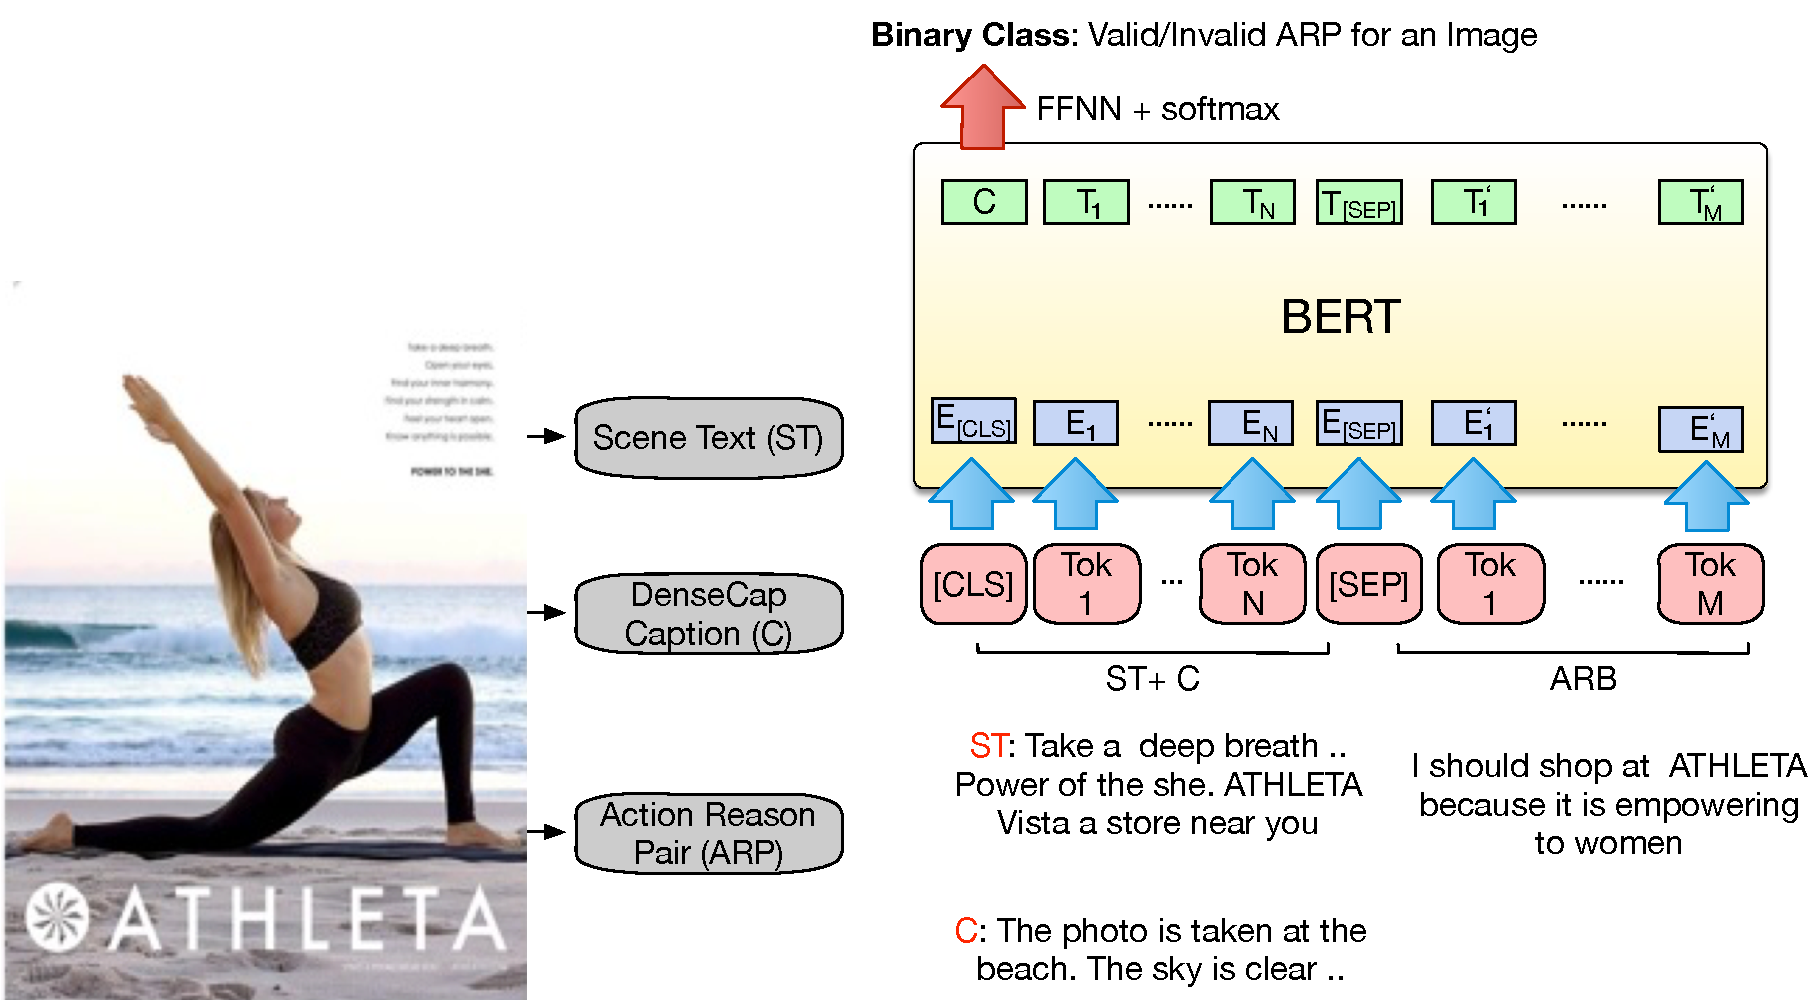
\includegraphics[width=0.6\textwidth]{BERT-2020.pdf}
%
%
%    \label{ActionButton}
%  \end{center}
%\end{figure}
\end{frame}
\BLOCK{endfor}


%\begin{frame}
%	\frametitle{A Sample Table}
%%\begin{itemize}
%
%
%
%
%
%
%%\end{itemize}
%\begin{block}{}
%\begin{table}
%\centering
%
%\resizebox{\columnwidth}{!}{
%\begin{tabular}{|l|c|c|c|c|}
%
%%\begin{tabularx}{\columnwidth}{|lcccc|}
%\hline
%
%\multicolumn{5}{|c|}{Unique Count of Textual Data}\\
%\hline
%\rowcolor{Gray}
%
% Dictionary & words  & nouns & verb & adjectives                        \\
% \hline
% %\rowcolor{Gray}
%%\multicolumn{5}{|c|}{Dictionary} \\
%% \hline
%Approach - model 1   &   00000000     &   00000000     & 00000000    & 00000000       \\   %\hdashline
%Approach - model  2  & 00000000 & 00000000 & 00000000 &  00000000  \\  %\hdashline
%  \hline
%
%
%\end{tabular}
%}
%%\end{tabularx}
%%\label{se:Dic}
%\end{table}
%\end{block}
%\note[item]{.}
%\end{frame}
%
%
%
%
%
%
%\begin{frame}[plain]{Mathematical Notation}
%\begin{alertblock}
%    {Equation 1}
%\begin{equation*}
%c_{t}=\sum_{j=1}^{T} \alpha_{t j} h_{j}, \alpha_{t j}=\frac{\exp \left(e_{t j}\right)}{\sum_{k=1}^{T} \exp \left(e_{t k}\right)}, e_{t j}=a\left(s_{t-1}, h_{j}\right)
%\end{equation*}
%
%
%\end{alertblock}
%
%
%
%
%\end{frame}
%
%
%\begin{frame}[noframenumbering,plain]
%\begin{center}
%\Huge \textcolor{cvut_blue}{Thank You}
%\end{center}
%\end{frame}


 \end{document}
% =============================================================
% =========================== END =============================
% =============================================================

